
\section{Final Product}
- detailed description about how the client and server app look like and how it works.

\subsection{Server-side application}

Maybe we can present milestones reached

\begin{figure}[H]
	\centering
		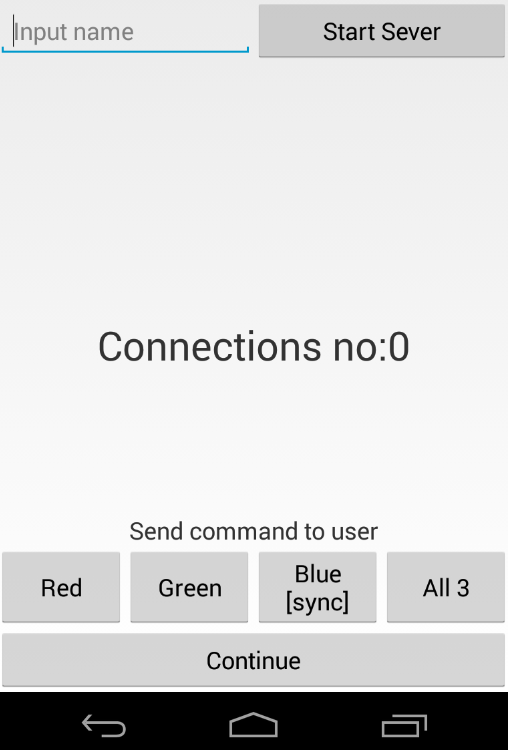
\includegraphics[width=5cm]{conclusion/server_ui.png}
	\caption{Server UI}
	\label{fig:Server_UI }
\end{figure}

\subsection{Client-side application}
\begin{figure}[H]
	\centering
		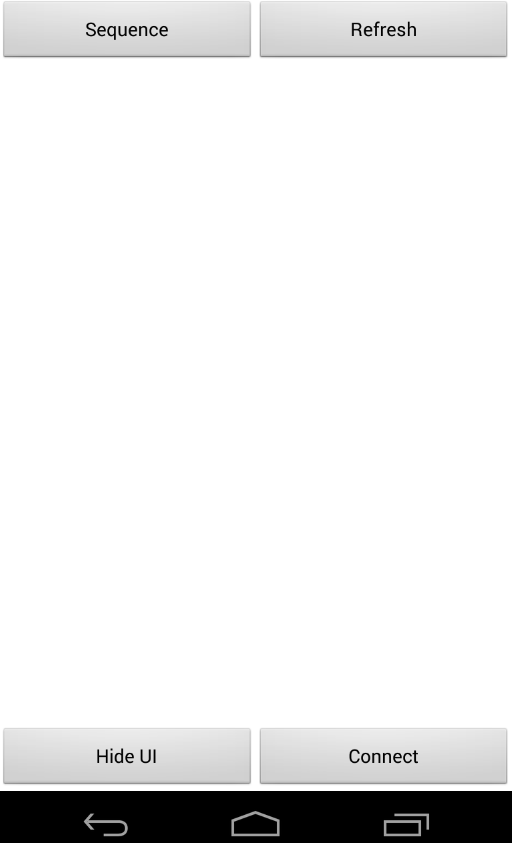
\includegraphics[width=7cm]{conclusion/user_ui.png}
	\caption{Client UI}
	\label{fig:Client_UI }
\end{figure}

\subsection{Functionalities}
???
%\section{Evaluation criteria}
%\section{Evaluation Results}
%\section{Conclusion}
%\section{Discussion}
\section{Further work}
performance, scalability


One of the first steps in further development is \emph{device tracking}.
Once the mobile device is detected, their position is saved but not updated during time.
It is probable, that on rock concerts, the audience wont be static, but 
device tracking

grid adjusting

improve image processing

jeden screen jako vice pixelu


\section{Summary}


- reflect on nonfunctional requirements